\section{Plasma, Tokamak Plasma and Tokamak Edge Plasma Modeling: Theory and Simulation}
    \BA{Introduction.}

    At its heart, a plasma is a fluid, albeit a multiphase, electrically-charged one. Constructing a plasma model therefore follows the same workflow as that of constructing a model for a typical single phase, non-electrically-charge fluid. Many of the assumptions that we would traditionally make when deriving traditional fluid model such as the Navier–Stokes equations (such as in particular the dominance of collisions in the Boltzmann equation \BA{[Ref]}) fail in the case of (tokamak) plasmas however. It makes sense therefore to return to the fundamentals, and construct our model from the ground up.

    \BA{Diagram of flow from particle to kinetic to fluid models, illustrating assumptions made at each step.}

    \BA{The good, the bad and the ugly of the plasma modeling world haha haha.}

    \subsection*{Particle Models}
    Perhaps the most fundamental mathematical model for a plasma is the particle model.
    \begin{definition}[Particle model]
        Here, ``particle'' models refer to those wherein every single particle is modelled individually.
    \end{definition}
    Supposing particle indexed via the index $i$ in a phase indexed via the index $s$, has position $\bfx_{si}(t)$ and velocity $\bfv_{si}(t)$, $(\bfx_{si})_{si}$ and $(\bfv_{si})_{si}$ satisfy the systems of ODEs:
    \begin{align}
        \bfd\bfx_{si}  &=  \bfv_{si} dt  \label{patricle motion}  \\
        m_{s}\bfd\bfv_{si}  &=  q_{s}[(\bfE - \bfE_{si}) + \bfv_{si}\wedge(\bfB - \bfB_{si})]dt  \label{particle forcing}
    \end{align}
    where $\bfE_{si}$, $\bfB_{si}$ refer to the contributions to the electric and magnetic fields (respectively) \emph{not} generated by the particle indexed $s$, $i$, satisfying Maxwell's equations:
    \begin{align*}
        \partial_{t}\bfE_{si}  &=  c^{2}\nabla\wedge\bfB_{si} - \frac{1}{\varepsilon_{0}}\sum_{s', i' : (s', i') \neq (s, i)}q_{s'}\delta^{3}(\bfx - \bfx_{s'i'})\bfv_{si},  &
        \partial_{t}\bfB_{si}  &=  - \nabla\wedge\bfE_{si}  \\
        \nabla\cdot\bfE_{si}  &=  \frac{1}{\varepsilon_{0}}\sum_{s', i' : (s', i') \neq (s, i)}q_{s'}\delta^{3}(\bfx - \bfx_{s'i'}),  &
        \nabla\cdot\bfB_{si}  &=  0
    \end{align*}
    Naturally this leads to the most complete dynamical model, however on the tokamak scale with particle densities on the order of $10^{- 5}{\rm mol}^{- 1}$ this is computationally impossible. We must therefore begin to make certain assumptions to simplify the model to bring it within reach of analysis.
    
    \subsection*{Kinetic Models}
    \begin{definition}[Kinetic model]
        Here, ``kinetic'' models refer to those wherein the distribution of particles positions and velocities is modelled through a single distribution function, as a function of both position and velocity.
    \end{definition}
    For each phase, $s$, we define the (1-particle) distribution function $(f_{s}(\bfx, \bfv; \bft))_{s}$
    \begin{equation}
        f_{s}(\bfx, \bfv; \bft)  :=  \sum_{i}\delta^{3}(\bfx - \bfx_{si})\delta^{3}(\bfv - \bfv_{si})
    \end{equation}
    While working with such $(f_{s})_{s}$ could \emph{in theory} be used to model all the particles exactly and simultaneously, variations of each $f_{s}$ in $\bfx$ occur on the length scale of the distances between particles, i.e. on the order of $10^{- 6}\rmm$ in a tokamak plasma. We would therefore need a mesh resolution on a similar (if not finer) length scale to capture the physical nature of each $f_{s}$. Again: computationally infeasible.

    Since, however, the \emph{precise} position of each particle is generally irrelevant to the general fluid behavior when not working on the atomic scale (in particular on tokamak plasma scales) the key idea of kinetic theory is to model this distribution function as a \emph{random} distribution, as one might do in Bayesian statistics to model a parameter that is known to be of fixed value as a random variable when full information on it is unknown. One defines the 1-particle distribution functions, denoted here as $\left(\widetilde{f_{s}}(\bfx, \bfv)\right)_{s}$, such that $\forall \phi(\bfx, \bfv)$,
    \begin{equation}
        \bbE\left\{\int_{\bfx, \bfv}f_{s}(\bfx, \bfv)\phi(\bfx, \bfv)\right\}
        \left(=  \sum_{i}\bbE\{\phi(\bfx_{si}, \bfv_{si})\}\right)
        =  \int_{\bfx, \bfv}\widetilde{f_{s}}(\bfx, \bfv)\phi(\bfx, \bfv)
    \end{equation}
    Similarly the electromagnetic field must be modeled as a random distribution, with $\widetilde{\bfE}$, $\widetilde{\bfB}$ defined, such that $\forall \bfphi(\bfx)$,
    \begin{align}
        \bbE\left\{\int_{\bfx}\bfE(\bfx)\cdot\bfphi(\bfx)\right\}  =  \int_{\bfx}\widetilde{\bfE}(\bfx)\cdot\bfphi(\bfx),  && 
        \bbE\left\{\int_{\bfx}\bfB(\bfx)\cdot\bfphi(\bfx)\right\}  =  \int_{\bfx}\widetilde{\bfB}(\bfx)\cdot\bfphi(\bfx)
    \end{align}
    We seek a model in $\left(\widetilde{f_{s}}\right)_{s}$, $\widetilde{\bfE}$, $\widetilde{\bfB}$ \emph{only}. To do so, one must consider also the 2-particle distribution functions, denoted here as $\left(\widetilde{f_{s_{1}}f_{s_{2}}}[(\bfx_{1}, \bfv_{1}), (\bfx_{2}, \bfv_{2})]\right)_{s_{1}s_{2}}$, defined such that $\forall \phi[(\bfx_{1}, \bfv_{1}), (\bfx_{2}, \bfrefv_{2})]$,
    \begin{multline}
        \bbE\left\{\int_{\bfx_{1}, \bfv_{1}}\int_{\bfx_{2}, \bfv_{2}}f_{s_{1}}(\bfx_{1}, \bfv_{1})f_{s_{2}}(\bfx_{2}, \bfv_{2})\phi[(\bfx_{1}, \bfv_{1}), (\bfx_{2}, \bfv_{2})]\right\}  \\
        \left(=  \sum_{i_{1}, i_{2}}\bbE\{\phi[(\bfx_{s_{1}i_{1}}, \bfv_{s_{1}i_{1}}), (\bfx_{s_{2}i_{2}}, \bfv_{s_{2}i_{2}})]\}\right)  \\
        =  \int_{\bfx_{1}, \bfv_{1}}\int_{\bfx_{2}, \bfv_{2}}\widetilde{f_{s_{1}}f_{s_{2}}}[(\bfx_{1}, \bfv_{1}), (\bfx_{2}, \bfv_{2})]\phi[(\bfx_{1}, \bfv_{1}), (\bfx_{2}, \bfv_{2})]
    \end{multline}
    These capture (some of) the nature of how the positions of particles are correlated with each other.
    
    Since attempting to then track the behavior of the 2-particle correlation functions requires tracking certain 3-particle correlation functions etc., one must approximate $\left(\widetilde{f_{s_{1}}f_{s_{2}}}\right)_{s_{1}s_{2}}$ in terms of $\left(\widetilde{f_{s}}\right)_{s}$.\footnote{This is often referred to as the ``\emph{closure problem}''.} To do so, we make the 2 following assumptions:
    \begin{itemize}
        \item  The ``\emph{molecular chaos hypothesis}'' holds as the distance between particles tends to infinity.
        \begin{definition}[Molecular chaos hypothesis]
            The ``molecular chaos hypothesis'' asserts that the velocity of colliding particles are uncorrelated. \BA{[Ref]}
        \end{definition}
        In our case this would surmount to the assumption that
        \begin{equation}
            \widetilde{f_{s_{1}}f_{s_{2}}}[(\bfx_{1}, \bfv_{1}), (\bfx_{2}, \bfv_{2})]  =  \widetilde{f_{s_{1}}}(\bfx_{1}, \bfv_{1})\widetilde{f_{s_{2}}}(\bfx_{2}, \bfv_{2})
        \end{equation}
        We assume that this holds as the distance between particles tends to infinity, i.e. roughly speaking, as $\|\bfx_{1} - \bfx_{2}\|  \rightarrow  \infty$,
        \begin{equation}
            \widetilde{f_{s_{1}}f_{s_{2}}}[(\bfx_{1}, \bfv_{1}), (\bfx_{2}, \bfv_{2})]  \sim  \widetilde{f_{s_{1}}}(\bfx_{1}, \bfv_{1})\widetilde{f_{s_{2}}}(\bfx_{2}, \bfv_{2})
        \end{equation}
    \end{itemize}

    \BA{I think I wanna put the precise derivation of the Boltzmann equations in an appendix.}

    To cast an equation from the exact deterministic form to one in these random distribution parameters, one can follow the workflow in Figure \ref{kinetic model construction workflow}.
    \begin{figure}[!h]
        \centering
        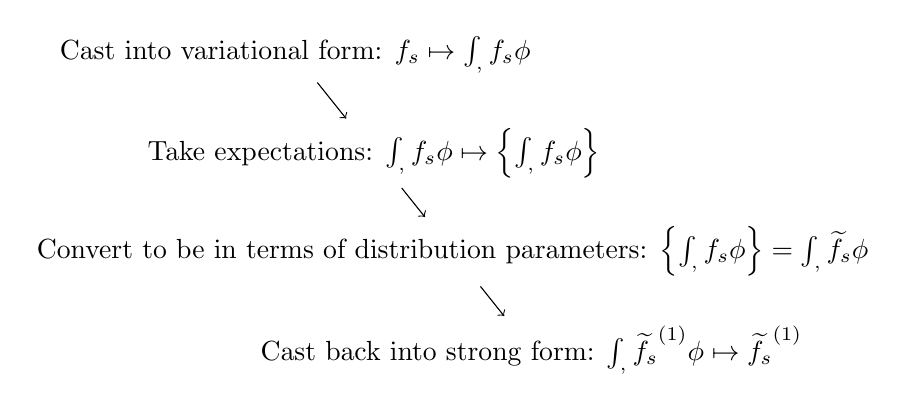
\begin{tikzpicture}[align = center, auto]
            \node (1) at (0, 0) {Cast into variational form: $f_{s}  \mapsto  \int_{\bfx, \bfv}f_{s}\phi$};
            \node (2) at (1, -1.25) {Take expectations: $\int_{\bfx, \bfv}f_{s}\phi  \mapsto  \bbE\left\{\int_{\bfx, \bfv}f_{s}\phi\right\}$};
            \node (3) at (2, -2.5) {Convert to be in terms of distribution parameters: $\bbE\left\{\int_{\bfx, \bfv}f_{s}\phi\right\}  =  \int_{\bfx, \bfv}\widetilde{f_{s}}\phi$};
            \node (4) at (3, -3.75) {Cast back into strong form: $\int_{\bfx, \bfv}\widetilde{f_{s}}^{(1)}\phi  \mapsto  \widetilde{f_{s}}^{(1)}$};

            \draw[->] (1) -- (2);
            \draw[->] (2) -- (3);
            \draw[->] (3) -- (4);
        \end{tikzpicture}
        \caption{Diagram of workflow for construction of a kinetic model}
        \label{kinetic model construction workflow}
    \end{figure}

    Since this is entirely linear, Maxwell's equations—themselves linear—carry over identically:
    \begin{align*}
        \partial_{t}\widetilde{\bfE}  &=  c^{2}\nabla\wedge\widetilde{\bfB} - \frac{1}{\varepsilon_{0}}\sum_{s}q_{s}\int_{\bfv}\widetilde{f_{s}}\bfv,  &
        \partial_{t}\widetilde{\bfB}  &=  - \nabla\wedge\widetilde{\bfE}  \\
        \nabla\cdot\widetilde{\bfE}  &=  \frac{1}{\varepsilon_{0}}\sum_{s}q_{s}\int_{\bfv}\widetilde{f_{s}},  &
        \nabla\cdot\widetilde{\bfB}  &=  0
    \end{align*}
    As for the evolution equations for $(f_{s})_{s}$ however, this is sadly \emph{not} the case, due to the non-linear forcing term. \BA{Introduce the 2-particle correlation functions!}

    \BA{Old text...}

    From equations (\ref{patricle motion}–\ref{particle forcing}), we see $(f_{s})_{s}$ satisfy the PDE
    \begin{equation}
        \partial_{t}f_{s} + \nabla_{\bfx}\cdot[f_{s}\bfv] + \frac{q_{s}}{m_{s}}\nabla_{\bfv}\cdot[f_{s}(\bfE + \bfv\wedge\bfB)]  =  0
    \end{equation}
    When considered in isolation, this is referred to as the ``Vlasov'' equation, and can be interpreted as a collision-less version of the Boltzmann equation (\BA{...}).

    \BA{Note here about dropping the tildes from here on out.}
    
    \subsection*{Fluid Models}
    \noindent\makebox[\linewidth]{\rule{\textwidth}{0.4pt}}
    \begin{definition}[Fluid model]
        Here, ``fluid'' models refer to those wherein the system is reduced from one in \emph{both} position and velocity space (and time) to one in \emph{just} position space (and time) through some kind of approximation to the distribution function.
    \end{definition}
    \noindent\makebox[\linewidth]{\rule{\textwidth}{0.4pt}}
    Recall the Boltzmann equation (\ref{eqn:Boltzmann equation})
    \begin{equation*}
        \partial_{t}f_{s} + \nabla_{\bfx}\cdot[f_{s}\bfv] + \frac{q_{s}}{m_{s}}\nabla_{\bfv}\cdot[f_{s}(\bfE + \bfv\wedge\bfB)]  =  \frac{q_{s}}{m_{s}}\sum_{s'}q_{s'}(\nabla_{\bfv}\cdot\bfC_{ss'})
    \end{equation*}
    To look at the dominant terms in this equation, one can non-dimensionalize. Denote the scale of a variable, $*$, with an overbar, $\overline{*}$. Suppose the following scales are given by the problem specification:
    \begin{align}
        \left(\overline{n}_{s}\right)_{s},        &&
        \overline{\bfx},                          &&
        \overline{\bfv},                          &&
        \overline{\bfB},                          &&
        \left(\overline{\bfC}_{ss'}\right)_{ss'}
    \end{align}
    where $n_{s}$ denote the particle density of species $s$,
    \begin{equation}
        n_{s}  :=  \int_{\bfv}f_{s}
    \end{equation}
    The remaining variable scales are given by:
    \begin{itemize}
        \item  $\overline{t}      =  \overline{\bfx}/\overline{\bfv}$, working on convective timescales.
        \item  $\overline{\bfE}   =  \overline{\bfv}\overline{\bfB}$, balancing the electric and magnetic Lorentz forces. \BA{(Why would this be the case?)}
        \item  $\overline{f}_{s}  =  \overline{n}_{s}/\overline{\bfv}^{3}$, by the definition of $n_{s}$.
    \end{itemize}
    
    The Boltzmann equation (\ref{eqn:Boltzmann equation}) then takes the non-dimensionalized form
    \begin{equation}
        \partial_{t}f_{s} + \nabla_{\bfx}\cdot[f_{s}\bfv] + \left\{\frac{q_{s}}{m_{s}}\cdot\frac{\overline{\bfx}\overline{\bfB}}{\overline{\bfv}}\right\}\nabla_{\bfv}\cdot[f_{s}(\bfE + \bfv\wedge\bfB)]  =  \sum_{s'}\left\{\frac{q_{s}q_{s'}}{m_{s}}\cdot\frac{\overline{\bfC}_{ss'}\overline{\bfx}\overline{\bfv}}{\overline{n_{s}}}\right\}(\nabla_{\bfv}\cdot\bfC_{ss'})
    \end{equation}
    
    Regarding the scale of these terms, consider the conditions during a JET reactor pulse, for a predominant (positive) deuterium \BA{(Should I be including tritium here?)} ion and (negative) electron phase, with physical parameters for the JET reactor as listed in Chapters 2 and 4 of \cite{Wes00}:
    \begin{itemize}
        \item  $\overline{n}_{\pm}        \approx  10^{19}\rmm^{- 3}$
        \item  $\overline{\bfx}           \approx  2.5\rmm$, twice the minor radius of $1.25\rmm$
        \item  $\overline{\bfv}           \approx  7.9\times 10^{5}\rmm\rms^{- 1}$, the thermal velocity $\sqrt{\rmk_{\rmB}T/\rmm_{+}}$ for the (mass/energy-dominant) ion phase at operational temperature $1.5\times 10^{8}\rmK$, in the middle of the range $1$–$2\times 10^{8}\rmK$
        \item  $\overline{\bfB}           \approx  3.5\rmT$
        \item  $\overline{\bfC}_{\pm\pm}  \approx  1.1\times 10^{25}\rms^{3}\rmT^{2}{\rm kg}^{- 1}\rmm^{- 5}$, from the approximation $\overline{\bfC}_{\pm\pm}  \approx  \overline{n}_{\pm}^{5/3}/\varepsilon_{0}\overline{\bfv}^{3}$ \BA{(Justification)}
    \end{itemize}
    The remaining scales then evaluate as:
    \begin{align}
        \overline{t}      \approx  3.2\times 10^{- 6}\rms,              &&
        \overline{\bfE}   \approx  2.8\times 10^{6}\rmT\rmm\rms^{- 1},  &&
        \overline{f_{s}}  \approx  2.1\times 10^{1}\rms^{3}\rmm^{- 6}
    \end{align}
    
    \BA{(Think I should be including a separate force for ion-ion/electron-electron repulsion...)} 
    
    The dimensionless constants $\left(q_{s}/m_{s}\cdot\overline{\bfx}\overline{\bfB}/\overline{\bfv}\right)_{s}$ therefore evaluate for each phase as:
    \begin{align}
        \frac{q_{+}\overline{\bfx}\overline{\bfB}}{m_{+}\overline{\bfv}}  &\approx  5.3\times 10^{2},   \\
        \frac{q_{-}\overline{\bfx}\overline{\bfB}}{m_{-}\overline{\bfv}}  &\approx  (-) 2.0\times 10^{6}
    \end{align}
    while the constants $\left(q_{s}q_{s'}/m_{s}\cdot\overline{\bfC}_{ss'}\overline{\bfx}\overline{\bfv}/\overline{n_{s}}\right)_{ss'}$ evaluate as:
    \begin{align}
        \frac{q_{+}q_{+}}{m_{+}}\cdot\frac{\overline{\bfC}_{++}\overline{\bfx}\overline{\bfv}}{\overline{n_{+}}}  \approx  \frac{q_{+}q_{-}}{m_{+}}\cdot\frac{\overline{\bfC}_{+-}\overline{\bfx}\overline{\bfv}}{\overline{n_{+}}}  &\approx  1.6\times 10^{1}  \\
        \frac{q_{-}q_{+}}{m_{-}}\cdot\frac{\overline{\bfC}_{-+}\overline{\bfx}\overline{\bfv}}{\overline{n_{-}}}  \approx  \frac{q_{-}q_{-}}{m_{-}}\cdot\frac{\overline{\bfC}_{--}\overline{\bfx}\overline{\bfv}}{\overline{n_{-}}}  &\approx   6.0\times 10^{4}
    \end{align}
    
    On the convective parameter scales of many plasmas, \BA{(What \emph{are} these parameter scales? Dimensional analysis!)} it is the case that these equations are dominated by those components of the collisional terms which are only affected by $(f_{s'}|_{\bfx})_{s'}$ \BA{(Really don't like the phrasing there...)}, $\bfC_{s}^{(0)}$, and the forcing terms, $\frac{q_{s}}{m_{s}}\nabla_{\bfv}\cdot[f_{s}\left(\bfE + \bfv\wedge\bfB\right)]$. Fluid models will often seek to exploit this fact to say that the system has a set of leading-order solutions, $\left(f_{s}^{(0)}\right)_{s}$, satisfying the leading-order PDEs
    \begin{equation}\label{eqn:Maxwellian equation}
        \frac{q_{s}}{m_{s}}\nabla_{\bfv}\cdot\left[f_{s}^{(0)}(\bfE + \bfv\wedge\bfB)\right]  =  \nabla_{\bfv}\cdot\left[\bfC_{s}^{(0)}\left(\left(f_{s'}^{(0)}|_{\bfx}\right)_{s'}\right)\right]
    \end{equation}
    Since, however, the leading-order collision operators $\left(\bfC_{s}^{(0)}\right)_{s}$ conserve both momentum and energy, i.e.
    \begin{align*}
        \bfzero  &=  \sum_{s}\int_{\bfv}\left(\nabla_{\bfv}\cdot\bfC_{s}^{(0)}\right)m_{s}\bfv  &  0  &=  \sum_{s}\int_{\bfv}\left(\nabla_{\bfv}\cdot\bfC_{s}^{(0)}\right)\frac{1}{2}m_{s}\|\bfv\|^{2}  \\
        &=  - \sum_{s}\int_{\bfv}\bfC_{s}^{(0)}m_{s}  &  &=  - \sum_{s}\int_{\bfv}\bfC_{s}^{(0)}\cdot m_{s}\bfv
    \end{align*}
    \BA{(I only accounted for \emph{kinetic} energy here, I didn't include the \emph{magnetic potential} energy- not sure if I need to? Would be a nice opportunity to define $\bfA$ if I do.)} equation (\ref{eqn:Maxwellian equation}) is not (necessarily) well-posed, as taking moments for momentum and energy,
    \begin{align*}
        \bfzero  &=  \sum_{s}\int_{\bfv}\frac{q_{s}}{m_{s}}\nabla_{\bfv}\cdot\left[f_{s}^{(0)}(\bfE + \bfv\wedge\bfB)\right]m_{s}\bfv  &  0  &=  \sum_{s}\int_{\bfv}\frac{q_{s}}{m_{s}}\nabla_{\bfv}\cdot\left[f_{s}^{(0)}(\bfE + \bfv\wedge\bfB)\right]\frac{1}{2}m_{s}\|\bfv\|^{2}  \\
        &=  - \sum_{s}\int_{\bfv}f_{s}^{(0)}(\bfE + \bfv\wedge\bfB)q_{s}  &  &=  - \sum_{s}\int_{\bfv}f_{s}^{(0)}(\bfE + \bfv\wedge\bfB)\cdot q_{s}\bfv  \\
        &=  - \rho_{C}\bfE - \bfj\wedge\bfB  &  &=  - \bfj\cdot\bfE
    \end{align*}
    representing the bulk forces and heating on each of the phases, where the charge and current density, $\rho_{C}$ and $\bfj$ respectively, are defined:
    \begin{align}
        \rho_{C}  :=  \sum_{s}\int_{\bfv}f_{s}q_{s},  &&
        \bfj      :=  \sum_{s}\int_{\bfv}f_{s}q_{s}\bfv
    \end{align}
    functions of $\bfx$, $t$ only.
    
    This can be resolved by adding the terms:
    \begin{align}
        \nabla_{\bfv}\cdot\left[f_{s}\frac{1}{\rho_{Ms}}(\rho_{C}\bfE + \bfj\wedge\bfB)\right],  &&
        \Delta_{\bfv}\left[f_{s}\frac{1}{\rho_{M}}\left(\bfE\cdot\left(\frac{\rho_{C}}{\rho_{M}}\bfp - \bfj\right) + \bfB\cdot(\bfp\wedge\bfj)\right)\right]
    \end{align}
    to equation (\ref{eqn:Maxwellian equation}).
    
    Define also the mass and momentum density, $\rho_{M}$ and $\bfp$ respectively:
    \begin{align}
        \rho_{C}  :=  \sum_{s}\int_{\bfv}f_{s}m_{s},  &&
        \bfp      :=  \sum_{s}\int_{\bfv}f_{s}m_{s}\bfv
    \end{align}
    and velocity density, $\bfu$,
    \begin{equation}
        \bfu  :=  \frac{1}{\rho_{M}}\bfp
    \end{equation}
    all functions of $\bfx$, $t$ \emph{only}.
    
    Rewriting the Boltzmann equation in the form
    {\small \begin{multline}
        \partial_{t}f_{s} + \nabla_{\bfx}\cdot[f_{s}\bfv] + \nabla_{\bfv}\cdot\left[f_{s}\frac{1}{\rho_{M}}(\rho_{C}\bfE + \bfj\wedge\bfB)\right] + \Delta_{\bfv}\left[f_{s}\frac{1}{\rho_{M}}\left(\bfE\cdot\left(\frac{\rho_{C}}{\rho_{M}}\bfp - \bfj\right) + \bfB\cdot(\bfp\wedge\bfj)\right)\right]  \\
        + \nabla_{\bfv}\cdot\left[f_{s}\frac{q_{s}}{m_{s}}(\bfE + \bfv\wedge\bfB)\right] - \nabla_{\bfv}\cdot\left[f_{s}\frac{1}{\rho_{M}}(\rho_{C}\bfE + \bfj\wedge\bfB)\right]  \\
        - \Delta_{\bfv}\left[f_{s}\frac{1}{\rho_{M}}\left(\bfE\cdot\left(\frac{\rho_{C}}{\rho_{M}}\bfp - \bfj\right) + \bfB\cdot(\bfp\wedge\bfj)\right)\right]  =  \nabla_{\bfv}\cdot[\bfC_{s}((f_{s'})_{s'})]
    \end{multline}}
    the leading-order system
    \begin{multline}
        \nabla_{\bfv}\cdot\left[f_{s}\frac{q_{s}}{m_{s}}(\bfE + \bfv\wedge\bfB)\right] - \nabla_{\bfv}\cdot\left[f_{s}\frac{1}{\rho_{M}}(\rho_{C}\bfE + \bfj\wedge\bfB)\right]  \\
        - \Delta_{\bfv}\left[f_{s}\frac{1}{\rho_{M}}\left(\bfE\cdot\left(\frac{\rho_{C}}{\rho_{M}}\bfp - \bfj\right) + \bfB\cdot(\bfp\wedge\bfj)\right)\right]  =  \nabla_{\bfv}\cdot\left[\bfC_{s}^{(0)}((f_{s'}|_{\bfx})_{s'})\right]
    \end{multline}
    \emph{does} admit solutions, which can be written as a function of just the functions in $\bfx$, t conserved by the collision operator, the density for each phase, total momentum and total energy:
    \begin{align}
        \rho_{Ms}  :=  \int_{\bfv}f_{s}m_{s},  &&
        \bfp  :=  \sum_{s}\int_{\bfv}f_{s}m_{s}\bfv,  &&
        E  :=  \sum_{s}\int_{\bfv}f_{s}\frac{1}{2}m_{s}\|\bfv\|^{2}
    \end{align}
    Assuming $f_{s}  \sim  f_{s}^{(0)}$ (i.e. that the plasma has ``thermalised'') and taking the above moments of the Boltzmann equation, we retrieve a system in $(\rho_{Ms})_{s}$, $\bfp$, $E$ only. This techniques allows the reduction of the system from one in the 6 (or 7) dimensions of a full kinetic model, to a fluid mode in just 3 (or 4).
    
    The problem however with applying this technique directly to tokamak plasmas fundamentally lies in the assumption of collision-dominant dynamics. \BA{(Some estimates on the scale of these terms in the plasma/edge plasma- some nice parameter scale estimates/values in that gyrokinetics manuscript- Multiscale Gyrokinetics for Rotating Tokamak Plasmas: Fluctuations, Transport and Energy Flows.)} Many highly influential so-called ``kinetic'' effects are not captured by these MHD fluid models, including: \BA{([Ref, Ref, Ref, …])}
    \begin{itemize}
        \item  Most plasma waves
        \item  Most plasma/kinetic instabilities
        \item  Landau damping/Bump-on-tail instabilities
        \item  Leakage
        \item  Kinetic structures (Beams/Double layers)
        \item  Anisotropic pressures
    \end{itemize}
    Techniques for the numerical solution of the MHD equations have been very well developed over recent years however \BA{([Ref, Ref, Ref, Ref, Ref, …])}. The question therefore lies in how these more efficient techniques, can be reapplied to the more accurate kinetic models, when the two are so qualitatively different.

    \BA{...whereby through some approximation to the 2-particle distribution functions, the collision terms, $(\bfC_{ss'})_{ss'}$, are written in terms of the 1-particle distribution functions, $(f_{s})_{s}$.}
    
    \BA{(Check out \href{https://upload.wikimedia.org/wikipedia/commons/a/a9/A_Comparison_Chart_For_Modeling_Plasma2.png}{this} diagram off Wikipedia, or again the content under ``Mathematical Descriptions'' \href{https://en.wikipedia.org/wiki/Plasma_(physics)}{here}.)}

    \BA{Would like to consider an expansion of the collision operator of the form
    \begin{multline}
        \bfC_{s}  =  \left[f_{s}\rho_{s'}(\bfmu_{ss'}(\bfu_{s'} - \bfv) + \nabla_{\bfx}\cdot[\bftau_{ss'}({\bf sym}(\nabla_{\bfx}\bfu_{s}))] + \cdots)\right]  \\
        + \nabla_{\bfv}\cdot\left[f_{s}\rho_{s'}(\bfD_{ss'}(\bfu_{s'} - \bfv) + \cdots)\right] + \cdots
    \end{multline}}
    
    \BA{I have some inconsistency in notation here with the rest of the paper in how I donate integrals. I should make this consistent, by denoting $\int_{\bfx}  \mapsto  \int_{\bfOmega}$ and, say, $\int_{\bfv}  \mapsto  \int_{\bfXi}$.}
    
    \BA{Change my $\rho_{M}$'s and $\rho_{C}$'s to $\rho_{\rmM}$'s and $\rho_{\rmC}$'s.}
    
    \BA{Not mentioned at all here that I'm discounting relativistic effects, and looking at the velocity scales that'd be quite a poignant remark.}
    
